\subsection{Stability over time}\label{sec:systemsresults}
A rolling-origin backtest refits each horizon's selected configuration on expanding windows and tests on 2021, 2022, 2023 and 2024.
The resulting relative MAE ranges are:
\begin{itemize}
  \item next report: 0.970--0.976;
  \item 3 days: 0.952--0.960;
  \item 7 days: 0.936--0.946;
  \item 14 days: 0.920--0.936.
\end{itemize}
These bracket the main test values, so the improvement over persistence is not an artefact of one test year.
The 2024 fold coincides with the validation year.

\subsection{Streaming}
We replayed \num{20000} real archived reports through a six-partition Kafka topic at 2,000 events/s with labelled faults: 5\% duplicates, 2\% late re-sends, 1\% malformed messages, and local reordering.
Of \num{21524} messages:
\begin{itemize}
  \item \num{20000} distinct events reached silver, with none missing and none never sent;
  \item \num{1317} duplicate or late copies were removed by watermarked de-duplication;
  \item 207 malformed messages were quarantined;
  \item none were dropped by the watermark.
\end{itemize}
The canonicalised streaming rows matched the batch canonicalisation of the same records in all 14 compared columns, with 0 mismatches.
The median per-batch producer-to-sink latency was 1.7\,s with a 2\,s trigger.
The red-team review found that an earlier version let a malformed message advance the event-time watermark and silently discard every later event. Unusable messages are now quarantined before the watermark, and a regression test covers this case.

\subsection{Storage and distributed execution}
The silver layer (692\,MB, \num{1743} files) was loaded into a three-DataNode HDFS with replication 3.
fsck reported no missing or corrupt blocks, and a file remained readable, with an identical checksum, while a DataNode was stopped.
All DataNodes share one physical disk, and there is a single NameNode.
On a containerised standalone Spark cluster (2 workers, 6 cores, 1\,GB executors) reading from HDFS, the aggregation workload processed 11.3M real rows in 9.2\,s and the window-feature workload in 14.4\,s.
These runs exercise the distributed code path (separate driver and executor JVMs, network shuffle, HDFS reads) but not multi-machine scaling.

\subsection{Single-host scalability}
\begin{figure}[t]
\centering
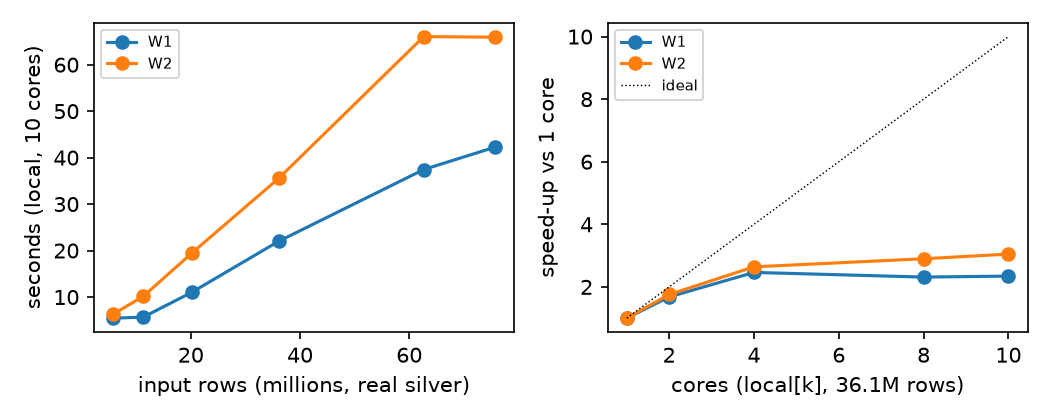
\includegraphics[width=0.9\linewidth]{scalability.png}
\caption{Left: run time against input size on the full silver layer (local mode, 10 cores). Right: speed-up against core count for 36.1M rows. W1 is an aggregation; W2 is per-entity window features.}\label{fig:scale}
\end{figure}
On one Apple M5 laptop (4 performance and 6 efficiency cores, 16\,GB), run time grows roughly linearly with input up to the full \num{75.6}M-row silver layer (Figure~\ref{fig:scale}).
Throughput is 1.6--2.0M rows/s for the aggregation and about 1.0M rows/s for the window features, with about 1\,GB of shuffle at full size and no disk spill.
Speed-up with cores flattens after four, matching the performance-core count: 2.5$\times$ for the aggregation and 3.0$\times$ for the window features at 10 cores.
The complete feature build for the forecasting panel (33M reports, 25 features, four targets) takes 8.3 minutes (\texttt{logs/f1\_build\_features.log}), and the full benchmark (38 model fits on 2M rows each, i.e.\ 32 candidates and 6 ablations, plus scoring of 6.4M test forecasts) takes 1\,h\,41\,min.
